\documentclass[12pt, letterpaper,]{article}
% for math
\usepackage{stix}
\usepackage{array}
\usepackage[portrait]{geometry}
\usepackage{t1enc}
\usepackage{mathptmx}
\usepackage{amsmath}
\usepackage{amsthm}
\usepackage[T1]{fontenc}
\usepackage{amsmath}
\usepackage{amssymb}
% for links in index
\usepackage[hidelinks]{hyperref}
\usepackage{url}
\usepackage{mathtools}
\newcommand\Mycomb[2][^m]{\prescript{#1\mkern-0.5mu}{}C_{#2}}
\newcommand\Mycombn[2][^n]{\prescript{#1\mkern-0.5mu}{}C_{#2}}
\newcommand\Mycombmn[2][^{m-1}]{\prescript{#1\mkern-0.5mu}{}C_{#2}}
% for para to start without indentation
\usepackage{ ragged2e }
\usepackage[parfill]{ parskip }

% for including figures
\usepackage{graphicx}
\usepackage{float}

% to set depth of table of contents to 1
\setcounter{tocdepth}{4}

% to make index
\usepackage{makeidx}

% to remove default section numbering
\setcounter{secnumdepth}{4}
% end preamble 
\begin{document}
\sffamily
\title{\Large{\textbf{Filter Design Assignment Elliptic}}\\
\author{}
               Tejaswee Sulekh-20D070082 \\ Filter Number=84}
\date{}
\maketitle 
\vspace{65mm}
\begin{center} \centering
\Large{\textbf{Group 26}}\\
    \large{Reviewer - Hemant Hajare}\\
    \Large{Department of Electrical Engineering}
\end{center}
\newpage
\tableofcontents
\newpage
\section{Student Details}
\textbf{Name:}\hspace{2.3cm} Tejaswee Sulekh\\
\textbf{Roll Number:}\hspace{1cm} 20D070082\\
\textbf{Filter Number:}\hspace{0.7cm} 84\\

\section{Analog Lowpass Elliptic}
We will have to get an analogous lowpass transfer function for both bandpass and bandstop requirements. Therefore, we need to design using \textbf{Elliptic} approximation. Since, the tolerance($\delta$) in both passband and stopband is 0.15. The transfer function is of the form: - 

\begin{equation}
    H_{analog,LPF}(S_L) = \frac{H_o}{D_o(S_L)}\prod\frac{s_L^2 + a_{0I}}{s_L^2 + b_{1i}s_L + b_{0i}}
\end{equation}

Where, 

\begin{figure}[!ht]
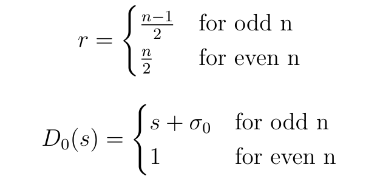
\includegraphics[width=8 cm]{Eq1.png}
\centering
\vspace{-3mm}
\end{figure}


\newpage
The transfer function coefficient and multiplier $H_o$ can be computed using the following formulae sequence:

\begin{figure}[!ht]
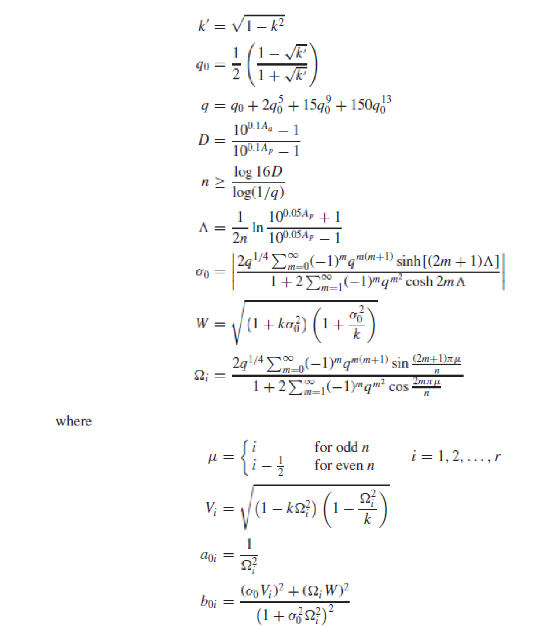
\includegraphics[width=13 cm]{Eq2.png}
\centering
\vspace{-3mm}
\end{figure}

\begin{figure}[!ht]
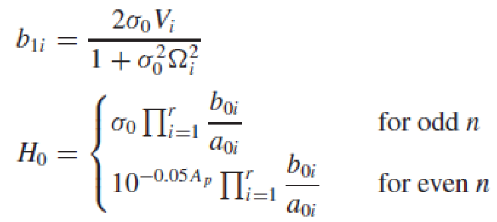
\includegraphics[width=5 cm]{Eq3.png}
\centering
\vspace{-3mm}
\end{figure}

\section{Filter-1(Bandpass) Details}
\subsection{Un-normalized Discrete Time filter Specifications}
Filter Number = 84\\
Therefore,\\
m = 4\\
q(m) = 0.1*4 = 0\\
r(m) = m - 10*q(m) = 4\\
BL(m) = 10 + 5*q(m) + 13*r(m) = 10 + 52 = 62 $Khz$\\
BH(m) = 75 + 62 = 137 $kHz$\\

Here, we have a analog signal with bandwidth of 280Khz. Where we sample it with 600Khz.

Here we have a bandpass filter with BL and BH (Khz)being the pass band frequencies for the filter to be designed. 

Hence, specifications here would be:
\begin{itemize}

\item \textbf{PassBand}: 62 to 137 Khz

\item \textbf{Transitionband}: 5Khz

\item \textbf{StopBand}: 0 to 57Khz and 142Khz to 300 Khz (As sampling frequency is 600 kHz)

\item \textbf{Tolerance}: 0.15 in magnitude for both Passband and Stopband

\item \textbf{Passband Nature}: Equiripple

\item \textbf{Stopband Nature}; Equiripple

\end{itemize}

\subsection{Normalized Digital Filter Specifications}

As we are sampling this signal at a frequency of 600 KHz. It is then normalized from 0 to   1$\pi$. By the following transformation:

\begin{equation}
    \omega = \frac{\Omega * 2 * \pi)}{\Omega_{s}(Sampling\_Rate)}
\end{equation}

Therefore the corresponding normalized discrete filter specifications are :-

\begin{itemize}

\item \textbf{PassBand}: $0.207\pi$ to $0.457\pi$

\item \textbf{Transitionband}: $0.0167\pi$

\item \textbf{StopBand}: $0 - 0.1899\pi$ to $0.4733\pi - 1\pi$

\item \textbf{Tolerance}: 0.15 in magnitude for both Passband and Stopband

\item \textbf{Passband Nature}: Equiripple

\item \textbf{Stopband Nature}; Equiripple

\end{itemize}
 
 \subsection{After applying bilinear transformation}

 The bilinear transformation is given as:

 \begin{equation}
     \Omega = tan(\frac{\omega}{2})
 \end{equation}

 \newpage

 From this transformation we end with the following new values:
\begin{table}[!h]
    \centering

\begin{tabular}{|c|c|}
\hline
Discrete & Analog \\
\hline
$0.207\pi$ & 0.3365 \\
$0.457\pi$ & 0.8723 \\
$0.0167\pi$ & 0.02618 \\
$0 - 0.1899\pi$ & 0 - 0.3076\\
$0.4733\pi - 1\pi$ & $0.9195 - \infty$ \\

\hline
\end{tabular}

\end{table}

Hence the corresponding frequencies will be as follows:

\begin{itemize}

\item \textbf{StopBand}: 0.3365 to 0.8723

\item \textbf{Transitionband}: 0.02618

\item \textbf{PassBand}: 0 to 0.3076 and 0.9195 to $\infty$

\item \textbf{Tolerance}: 0.15 in magnitude for both Passband and Stopband

\item \textbf{Passband Nature}: Equiripple

\item \textbf{Stopband Nature}: Equiripple

\section{Elliptical Bandpass Filter}
We need to use the same specifications which was there for the 1st filter
\begin{align*}
    B = 0.5358\\
    \Omega_0 = 0.5418\\
    \Omega_{LP} = 1\\
    \Omega_{LS} = 1.1203
\end{align*}
Consider $G_p$ = 0.85 and $G_s$ = 0.15\\
The value of K = $\frac{W_p}{W_s}$ = 0.8926\\
The value of K1 = $\frac{\sqrt{1/G_p^2-1}}{\sqrt{1/G_s^2-1}}$ =0.094
The minimum value of N after solving the elliptical integral of K,K1\\
\begin{align*}
    \lceil \frac{K_{1p}K}{K_pK_1}\rceil = 4
\end{align*}
Next we calculate the analog low pass transfer function\\
\begin{align*}
    \frac{0.85\,{\left(0.3196\,s^2 +1.0\right)}\,{\left(0.8835\,s^2 +1.0\right)}}{{\left(1.6\,s^2 +1.131\,s+1.0\right)}\,{\left(1.0\,s^2 +0.06192\,s+1.0\right)}}
\end{align*}
We now use the inverse transformation to convert the equivalent Elliptic low-pass
transfer function to get the Band-pass transfer function using the relation:-
\begin{align*}
    s_L = \frac{s^2+\Omega_0^2}{B\Omega}
\end{align*}
The analog band-pass transfer function:-\\
Numerator:-\\
$\text{1.7e+21}\,s^8 +\text{3.978e+21}\,s^6 +\text{3.113e+21}\,s^4 +\text{9.372e+20}\,s^2 +\text{9.437e+19}$\\


The denominator is:-\\
\begin{align*}
\text{2.0e+21}\,s^8 \\+\text{1.373e+21}\,s^7 \\+\text{5.651e+21}\,s^6 \\+\text{2.469e+21}\,s^5\\ +\text{4.895e+21}\,s^4 \\+\text{1.198e+21}\,s^3 \\+\text{1.331e+21}\,s^2 \\+\text{1.571e+20}\,s\\+\text{1.116e+20}
\end{align*}

We now make use of the Bilinear Transformation to convert the analog bandpass
filter into a discrete bandpass filter in the normalized angular frequency domain. The transform is as follows
\begin{align*}
    s = \frac{1-z^{-1}}{1+z^{-1}}
\end{align*}
Hence the Discrete Bandpass transfer function is:-\\
Numerator:-
\begin{align*}
    \text{1.965e+6}\,z^8 \\\text{- 5.002e+6}\,z^7 \\+\text{1.149e+7}\,z^6 \\\text{-1.555e+7}\,z^5 \\+\text{1.903e+7}\,z^4 \\\text{-1.555e+7}\,z^3 \\+\text{1.149e+7}\,z^2 \\\text{-5.002e+6}\,z\\+\text{1.965e+6}
\end{align*}
Denominator is :-
\begin{align*}
    \text{3.837e+6}\,z^8 \\\text{-8.446e+6}\,z^7 \\+\text{1.631e+8}\,z^6 \\\text{- 1.958e+7}\,z^5 \\+\text{2.146e+7}\,z^4 \\\text{- 1.582e+7}\,z^3 \\+\text{1.067e+7}\,z^2\\ \text{- 4.511e+6}\,z\\+\text{1.758e+6}
\end{align*}
\newpage
The frequency response is:-
\begin{figure}[!ht]
\frame{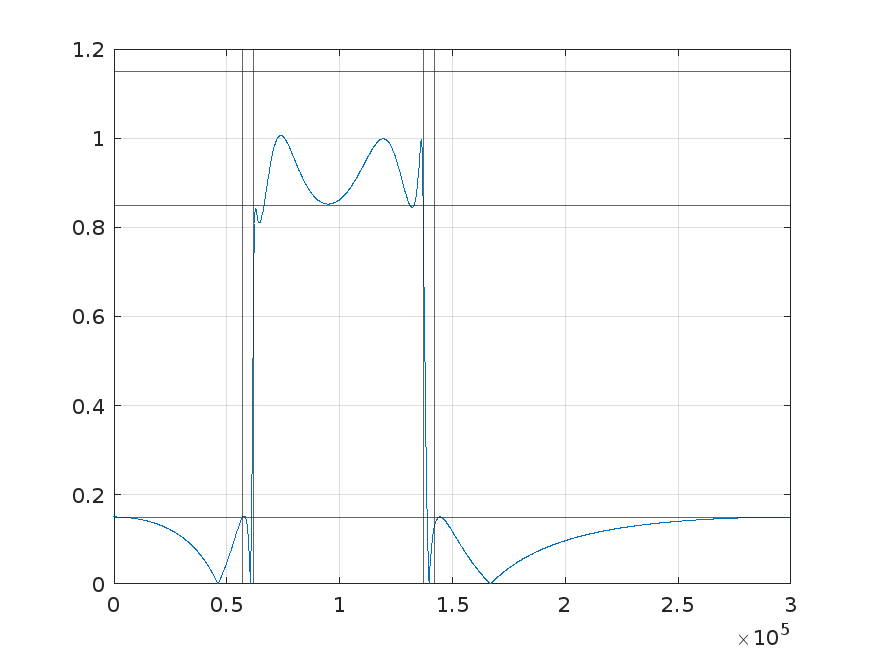
\includegraphics[width=10 cm]{Images/elip_freq.png}}
\centering
\vspace{-3mm}
\caption{Frequency response}
\end{figure}
\begin{figure}[!ht]
\frame{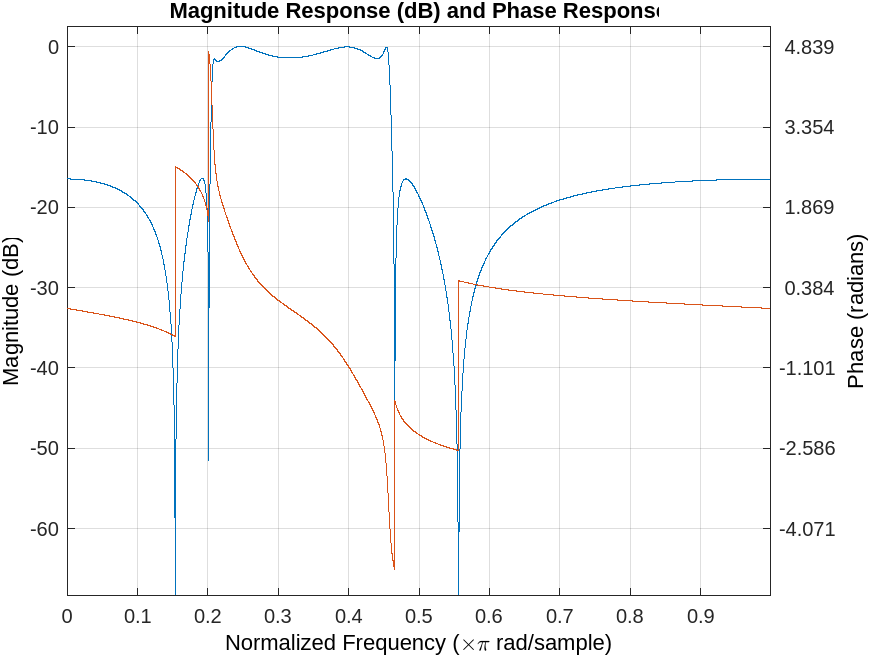
\includegraphics[width=10 cm]{Images/phasemagelip.png}}
\centering
\vspace{-3mm}
\caption{Magnitude and phase response}
\end{figure}
\begin{figure}[!ht]
\frame{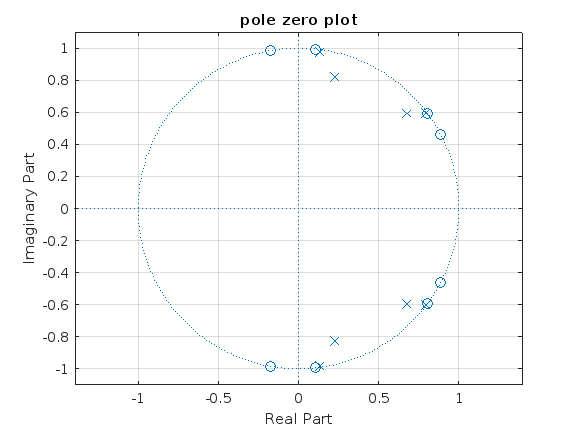
\includegraphics[width=10 cm]{Images/elip_poles.png}}
\centering
\vspace{-3mm}
\caption{Pole zero plot}
\end{figure}
\newpage
\end{itemize}


\section{Filter Details BandStop} %<--  Inngangur / Introduction

Calculations and detailed step-wise description is given below.

\subsection{Un-normalized discrete time filter specs}

Filter Number = 84
Therefore, m = 4
q(m) = 0
r(m) = 4
BL(m) = 64
BH(m) = 104

Here, we have a analog signal with bandwidth of 200Khz. Where we sample it with 425Khz.

Here we have a bandstop filter with BL and BH (Khz)being the stop band frequencies for the filter to be designed. 

Hence, specifications here would be:
\begin{itemize}

\item \textbf{StopBand}: 64 to 104 Khz

\item \textbf{Transitionband}: 5Khz

\item \textbf{PassBand}: 0 to 59Khz and 109Khz to 200Khz

\item \textbf{Tolerance}: 0.15 in magnitude for both Passband and Stopband

\item \textbf{Passband Nature}: Equiripple

\item \textbf{Stopband Nature}; Equiripple

\end{itemize}

\subsection{Normalized Digital Filter Specifications}

As we are sampling this signal at a frequency of 425 KHz. It is then normalized from 0 to $2\pi$. By the following transformation:

\begin{equation}
    \omega = \frac{\Omega * 2 * \pi)}{\Omega_{s}(Sampling\_Rate)}
\end{equation}

Therefore the corresponding normalized discrete filter specifications are :-

\begin{itemize}

\item \textbf{StopBand}: $0.325\pi$ to $0.4894\pi$

\item \textbf{Transitionband}: $0.0235\pi$

\item \textbf{PassBand}: $0 - 0.301\pi$ to $0.5129\pi - 1\pi$

\item \textbf{Tolerance}: 0.15 in magnitude for both Passband and Stopband

\item \textbf{Passband Nature}: Equiripple

\item \textbf{Stopband Nature}; Equiripple

\end{itemize}
 
 \subsection{After applying bilinear transformation}

 The bilinear transformation is given as:

 \begin{equation}
     \Omega = tan(\frac{\omega}{2})
 \end{equation}

 From this transformation we end with the following new values:
\begin{table}[!h]
    \centering

\begin{tabular}{|c|c|}
\hline
Discrete & Analog \\
\hline
$0.325\pi$ & $0.5594$ \\
$0.4894\pi$ & $0.96727$ \\
$0.0235\pi$ & $0.0369$ \\
$0 - 0.301\pi$ & $0 - 0.5118$\\
$0.5129\pi - 1\pi$ & $1.041 - \infty$ \\
\hline
\end{tabular}

\end{table}

Hence the corresponding frequencies will be as follows:

\begin{itemize}

\item \textbf{StopBand}: 0.5118 to 0.96727

\item \textbf{Transitionband}: 0.0369

\item \textbf{PassBand}: 0 to 0.466 and 1.041 to $\infty$

\item \textbf{Tolerance}: 0.15 in magnitude for both Passband and Stopband

\item \textbf{Passband Nature}: Equiripple

\item \textbf{Stopband Nature}; Equiripple

\end{itemize}

\subsection{Frequency Transformation and Relevant Parameters}

We need to transform the analog bandstop filter to an analog low-pass filter so that we can apply \textbf{Equiripple} filter design on it as both passband and stopband have equiripple nature. This is performed by using the following transformation.

\begin{equation}
    \Omega_{L} = \frac{B*\Omega}{\Omega_{o}^2 - \Omega^2}
\end{equation}

Where the two parameters above depend on the band pass frequencies in the following way:

$$\Omega_{o} = \sqrt{\Omega_{P_1}*\Omega_{P_2}} = \sqrt{0.466 * 1.041} = 0.57544$$
$$ B = \Omega_{P_2} - \Omega_{P_1} = 1.041 - 0.466 = 0.69670$$

\begin{table}[!h]
    \centering

\begin{tabular}{|c|c|}
\hline
$\Omega$ & $\Omega_L$\\
\hline
$0^+$ & $0^+$ \\
$0.466$ &  $+1 (\Omega_{L_{S_1}})$\\
$0.5118$ & $1.3184 (\Omega_{L_{P_1}})$\\
$0.7299$ &  $\infty$\\
$0.72994$ &  $-\infty$\\
$0.96727$ & $-1.23631(\Omega_{L_{S_2}})$\\
$1.041$ & $-1 (\Omega_{L_{P_2}})$\\
$\infty$ & $0^-$ \\
\hline
\end{tabular}

\end{table}

\subsection{Frequency Transformed Lowpass Analog filter specification}

\begin{itemize}
    \item \textbf{Passband Edge}: $1 (\Omega_{LP})$
    \item \textbf{Stopband Edge}: $\min(\Omega_{LS1},-\Omega_{LS2}) = \min(1.23621, 1.321) = 1.23621 (\Omega_{LS})$
    \item \textbf{Tolerance}: $0.15$ in magnitude for both Passband and Stopband
    \item \textbf{Passband Nature}: Equirriple
    \item \textbf{Stopband Nature}: Equirriple
\end{itemize}

\section{Elliptical Bandstop filter}
We need to use the same specifications which was there for the 2nd filter
\begin{align*}
    B = 0.57544\\
    \Omega_0 = 0.6967\\
    \Omega_{LP} = 1\\
    \Omega_{LS} = 1.23621
\end{align*}
Consider $G_p$ = 0.85 and $G_s$ = 0.15\\
The value of K = $\frac{W_p}{W_s}$ = 0.8726\\
The value of K1 = $\frac{\sqrt{1/G_p^2-1}}{\sqrt{1/G_s^2-1}}$ =0.094
The minimum value of N after solving the elliptical integral of K,K1\\
\begin{align*}
    \lceil \frac{K_{1p}K}{K_pK_1}\rceil = 4
\end{align*}
Next we calculate the analog low pass transfer function\\
\begin{align*}
\frac{0.6295\,s^2 +1.0}{{\left(1.605\,s+1.0\right)}\,{\left(0.9994\,s^2 +0.2305\,s+1.0\right)}}
\end{align*}
We now use the inverse transformation to convert the equivalent Elliptic lowpass
transfer function to get the Bandpstop transfer function using the relation:-
\begin{align*}
    s_L = \frac{B\Omega}{s^2+\Omega_0^2}
\end{align*}
The analog bandstop transfer function:-\\
Numerator:-\\
\begin{align*}
    \text{1.0e+15}\,s^6 +\text{1.665e+15}\,s^4 +\text{8.08e+14}\,s^2 +\text{1.144e+14}\\
\end{align*}
The denominator is:-\\
\begin{align*}
\text{1.0e+15}\,s^6 +\text{1.056e+15}\,s^5 +\text{1.91e+15}\,s^4 +\text{1.331e+15}\,s^3\\ +\text{9.269e+14}\,s^2 +\text{2.488e+14}\,s +\text{1.144e+14}\\
\end{align*}

We now make use of the Bilinear Transformation to convert the analog bandstop
filter into a discrete bandstop filter in the normalized angular frequency domain. The transform is as follows
\begin{align*}
    s = \frac{1-z^{-1}}{1+z^{-1}}
\end{align*}
Hence the Discrete Bandpass transfer function is:-\\
Numerator is:-
\begin{align*}
\text{3.587e+5}\,z^6 \text{-7.027e+5}\,z^5 +\text{1.424e+6}\,z^4 \text{-1.429e+6}\,z^3\\ +\text{1.424e+6}\,z^2 \text{-7.027e+5}\,z +\text{3.587e+5}\\
\end{align*}  

Denominator:- 
\begin{align*}
\text{6.587e+5}\,z^6 \text{-1.051e+6}\,z^5 +\text{1.641e+6}\,z^4 \text{-1.378e+6}\,z^3\\ +\text{1.135e+6}\,z^2 \text{-4.05e+5}\,z +\text{1.315e+6}\\
\end{align*}
The frequency response is:-
\begin{figure}[!ht]
\frame{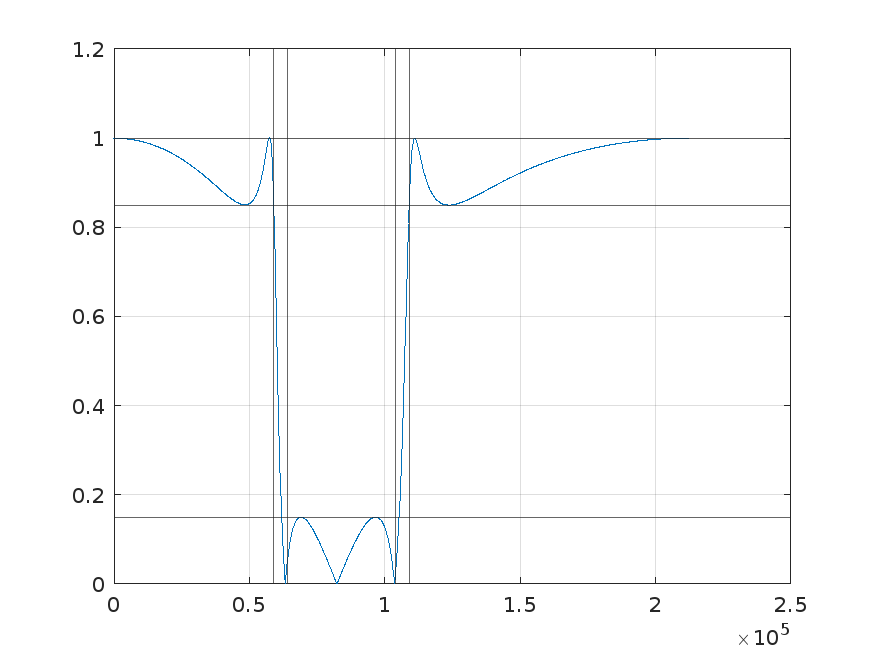
\includegraphics[width=10cm]{Images/Elliptical_bandstop.png}}
\centering
\vspace{-3mm}
\caption{Frequency response}
\end{figure}
\newpage
The magnitude and phase responses are
\begin{figure}[!ht]
\frame{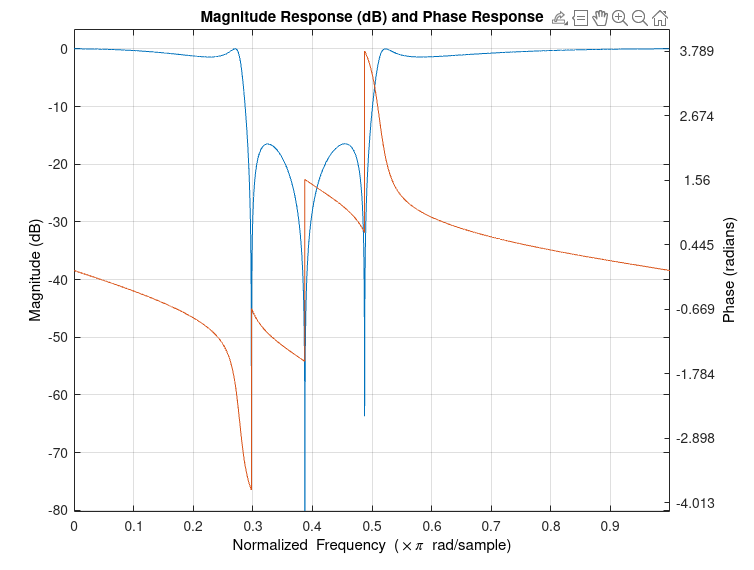
\includegraphics[width=10 cm]{Images/stopphase.png}}
\centering
\vspace{-3mm}
\caption{Magnitude and phase response}
\end{figure}\\
\begin{figure}[!ht]
\frame{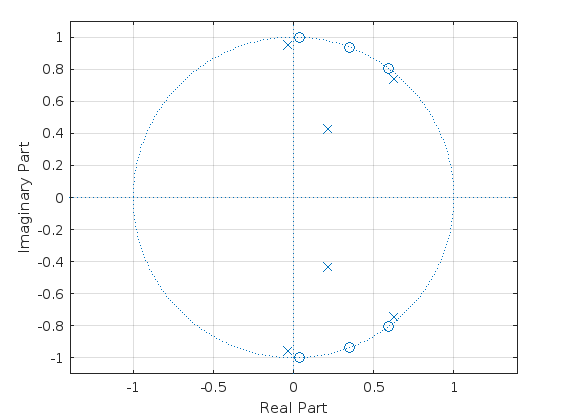
\includegraphics[width=10 cm]{Images/polesstop.png}}
\centering
\vspace{-3mm}
\caption{Pole zero plot}
\end{figure}\\
\newpage
\section{Comparison between Elliptical, Butterworth, Chebyshev filters}
\begin{itemize}
    \item The elliptic filter has the sharpest transition from passband to stopband or vice versa for the same specifications.
    \begin{align*}
         Elliptic > Chebyshev > Butterworth > Kaiser FIR
    \end{align*}
    \item We can see that the least resources required were in Elliptical filter, as compared to Butterworth and Chebyshev. The increasing order of resources:-
    \begin{align*}
        Elliptic (3) < Chebyshev (5) < Butterworth (22) < Kaiser FIR (100+)
    \end{align*}
    
    \item The FIR realisation gives the most linear phase response in the passband region. The increasing order of linearity
    \begin{align*}
        Elliptic < Chebyshev < Butterworth < Kaiser FIR
    \end{align*}
\end{itemize}

\textbf{All the codes are in the zip file along with this report}
\end{document}
